%%%%%%%%%%%%%%%%%%%%%%%%%%%%%%%%%%%%%%%%%%%
%                                         %
% This file should only be made of \input %
%                                         %
%%%%%%%%%%%%%%%%%%%%%%%%%%%%%%%%%%%%%%%%%%%

\chapter{Le client}

	\paragraph{}La partie client de notre application sert à interagir avec 
l'utilisateur humain. Basiquement, l'utilisateur tape des commandes et le 
client lui renvoie un résultat calculé par le daemon.
	
	\section{Architecture logique du client}

La figure \ref{client} illustre l'architecture de notre client. Tout d'abord, 
le client se charge de créer une socket permettant de se connecter à son daemon
, avec l'IP et le port adéquat. Il crée ensuite un thread qui s'occupe de gérer
 l'envoi des commandes tapées par l'utilisateur, en exécutant la fonction 
\verb"send_cmd()". Cette fonction crée elle aussi un thread qui, par le biais 
de la fonction \verb"recv_resp()", s'occupe d'afficher à l'écran les réponses 
aux commandes reçues du daemon.

\begin{center}
\begin{figure}[h]
    \centering
    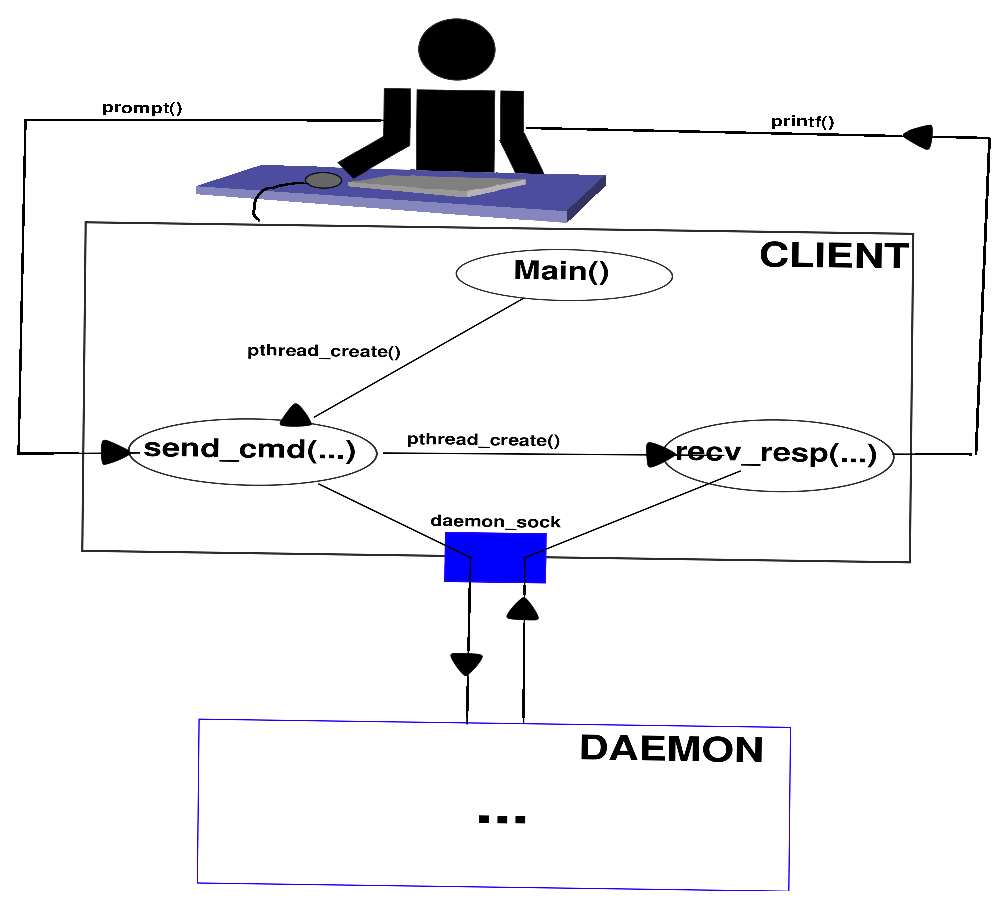
\includegraphics[scale=1.4]{client/archi_client.eps}
    \caption{Architecture du client}
    \label{client}
\end{figure}
\end{center}
	
	\section{Gestion des requ\^etes}

Le client s'occupe uniquement de renvoyer à l'utilisateur les réponses reçues
du daemon. En conséquence, l'intégralité des requêtes utilisateurs ne sont pas 
gérées directement par la partie client de notre application, mais par le 
daemon.
	
	\section{Implémentation actuelle}

Actuellement, notre application gère les requêtes utilisateur suivantes :
\begin{itemize}
\item \verb"help" : affiche une aide
\item \verb"list [options]" : donne la liste des ressources disponibles sur le 
      réseau sous la forme: \verb"cle nom taille \n"
\item \verb"info" : affiche des informations/statistiques sur l'état du 
      programme.
\item \verb"connect ip:port" : indique au programme de se connecter à un autre 
      programme
\item \verb"raw ip:port cmd" : envoie la commande de protocole cmd à un 
      programme. 
\end{itemize}

D'après la documentation, l'application doit être également capable de gérer 
les requêtes suivantes :
\begin{itemize}
\item \verb"set" : fournit la liste des options disponibles dans le programme
\item \verb"set option=valeur" : modifie la valeur d'une option
\item \verb"get cle" : récupère la ressource cle
\item \verb"download" : affiche des informations sur les fichiers en cours de 
      récupération (format libre)
\item \verb"upload" : affiche des informations sur les fichiers en cours de 
      transfert (format libre)
\end{itemize}
	
	\paragraph{}La simplicité de l'interface utilisateur, que l'on appelle 
	abusivement « client », est liée au fait que la plupart des actions 
	entreprises par le logiciel sont communes à tous les utilisateurs, 
	bien que souvent à l'initiative d'un unique utilisateur. L'intelligence 
	du logiciel, et en particulier la gestion des échanges de fichiers,
	est concentrée dans notre « démon », que nous allons décrire ci-dessous.
